\section{Introduction}
Since Einstein introduced the theory of general relativity in 1915 \cite{Einstein1915}, 
it has matched well with all experimental tests to date\cite{Will2014,Yunes2025GWTests}. 
General relativity has fundamentally transformed our understanding of space and time, 
explaining phenomena ranging from the anomalous precession of Mercury to the operation 
of atomic clocks in GPS satellites\cite{Ashby2003}, and predicting the existence of compact objects 
such as neutron stars and black holes, as well as gravitational waves \cite{Carroll2004,MisnerThorneWheeler1973,Einstein1916GW}.

Gravitational waves were first directly detected by LIGO in 2015 \cite{Abbott2016b}. 
These signals originate from some of the most energetic events in the universe, such as mergers of neutron stars and black holes. 
However, the signals detected by LIGO are extremely weak; the detectors are sensitive enough to measure relative length changes 
on the order of $10^{ 21}$, corresponding to displacements smaller than a proton diameter \cite{LIGO_Facts}. 
Despite this extraordinary sensitivity, gravitational wave signals remain weak relative to background noise. 
The highest signal to noise ratio (SNR) gravitational wave event reported to date is GW250114,
with a network matched filter SNR of approximately $80$ \cite{Abac2025GW250114}.

Interpreting gravitational wave detections requires accurate theoretical models of the expected signals. In practice, this is achieved by comparing observational data against waveform templates constructed from a combination of analytical approximations, phenomenological models, and numerical simulations. This template based comparison allows the physical properties of the source, including the component masses and spins, to be inferred statistically \cite{Veitch2015,Khan2016_IMRPhenomD}. Figure~\ref{fig:ligo_detector} shows an example of a gravitational wave detection matched to a numerical relativity waveform.

\begin{figure}[t]
    \centering
    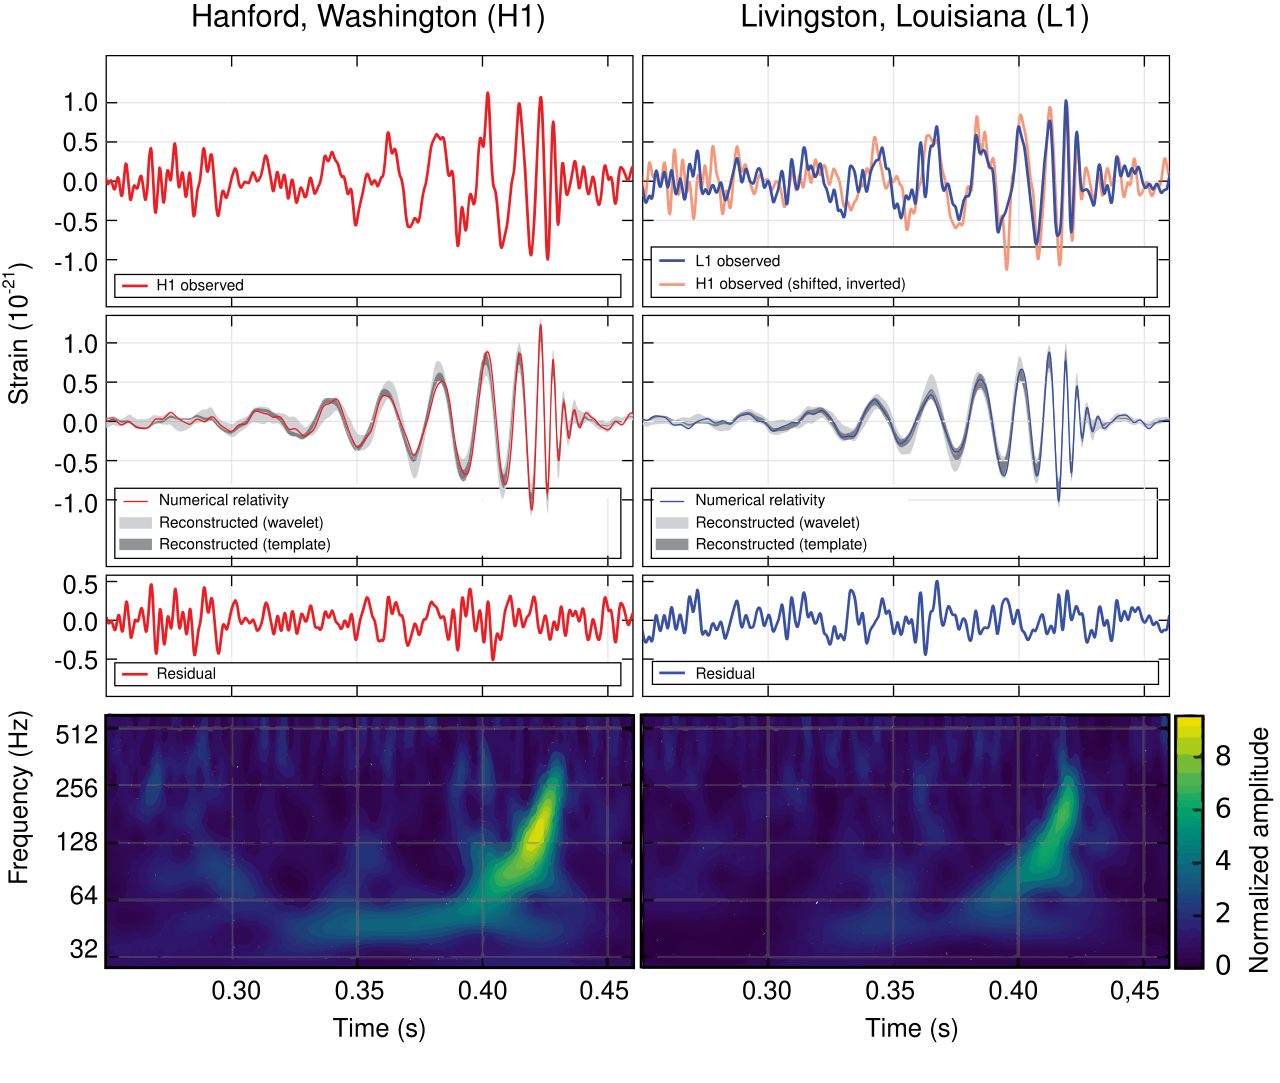
\includegraphics[width=0.8\textwidth]{Figures/LIGO_measurement_of_gravitational_waves.svg.png}
    \caption{Example of a gravitational wave signal detected by LIGO. The observed signal is compared with numerical relativity waveforms to identify the source as a binary black hole merger.}
    \label{fig:ligo_detector}
\end{figure}

Constructing theoretical models of binary black hole mergers is challenging because the relevant dynamics are strongly nonlinear and only partially accessible through analytic methods. In general relativity, exact analytic solutions are typically restricted to highly symmetric systems and cannot describe the full inspiral, merger, and ringdown of a generic binary black hole system. Numerical relativity therefore plays an essential role in modeling the late inspiral, merger, and ringdown, where fully nonlinear effects are important. A number of numerical relativity codes have been developed for this purpose, including the Einstein Toolkit, SpEC, GRChombo, BAM, GR Athena++, and Dendro GR \cite{Loffler2012,Boyle2019,Brugmann2008,Clough2015,Daszuta2021_GRAthena,Fernando2023}.

Simulating binary black hole mergers is computationally demanding. These simulations require solving a coupled system of nonlinear partial differential equations in three spatial and one time dimension, across multiple length scales, including the scale of the individual black holes, the orbital scale of the binary, and the radiation zone where gravitational waves are extracted \cite{BaumgarteShapiro2010,BaumgarteShapiro2021}. In this work, we make use of the Dendro numerical relativity framework, which combines adaptive mesh refinement with scalable parallel algorithms for binary black hole simulations \cite{Fernando2019,Fernando2019b,Fernando2023}.

For standard general relativity (GR), substantial progress has been made in modeling binary black hole mergers, and extensive
waveform catalogs now cover much of the binary black hole parameter space. In GR, the parameter space for binary black holes covers spin and mass ratio. Current catalogs have
good coverage for near equal mass systems. Here we define the mass ratio as
$q=M_{\mathrm{larger}}/M_{\mathrm{smaller}}\ge 1$. The LIGO  Virgo  KAGRA
(LVK) collaboration has reported hundreds of compact binary candidates using waveform
models informed by numerical relativity
\cite{Abbott2019,GWTC3,GWTC4,Boyle2019}.Future gravitational wave detectors, such as the Einstein Telescope and Cosmic Explorer, are expected to achieve significantly greater sensitivity than current ground based detectors \cite{Maggiore2020_ET,Reitze2019_CosmicExplorer,Evans2021_CEHorizon}. This increased sensitivity is expected to improve the signal to noise ratios of observed compact binary signals and to expand the range over which such systems can be detected. Meeting this challenge will require higher fidelity numerical simulations and more accurate waveform models \cite{Purrer2020_AccuracyRequirements,Black2025_ORBIT}.


In general, higher fidelity simulations, particularly those with larger mass ratios, require
finer grid resolution and therefore substantially greater computational cost. This trend is
illustrated in Fig.~\ref{fig:walltime}. Current simulations with mass ratios $q<8$ can
require weeks of runtime on modern supercomputers, and further increases in resolution
would significantly amplify this cost \cite{Boyle2019,Black2025_ORBIT}.

\begin{figure}[t]
    \centering
    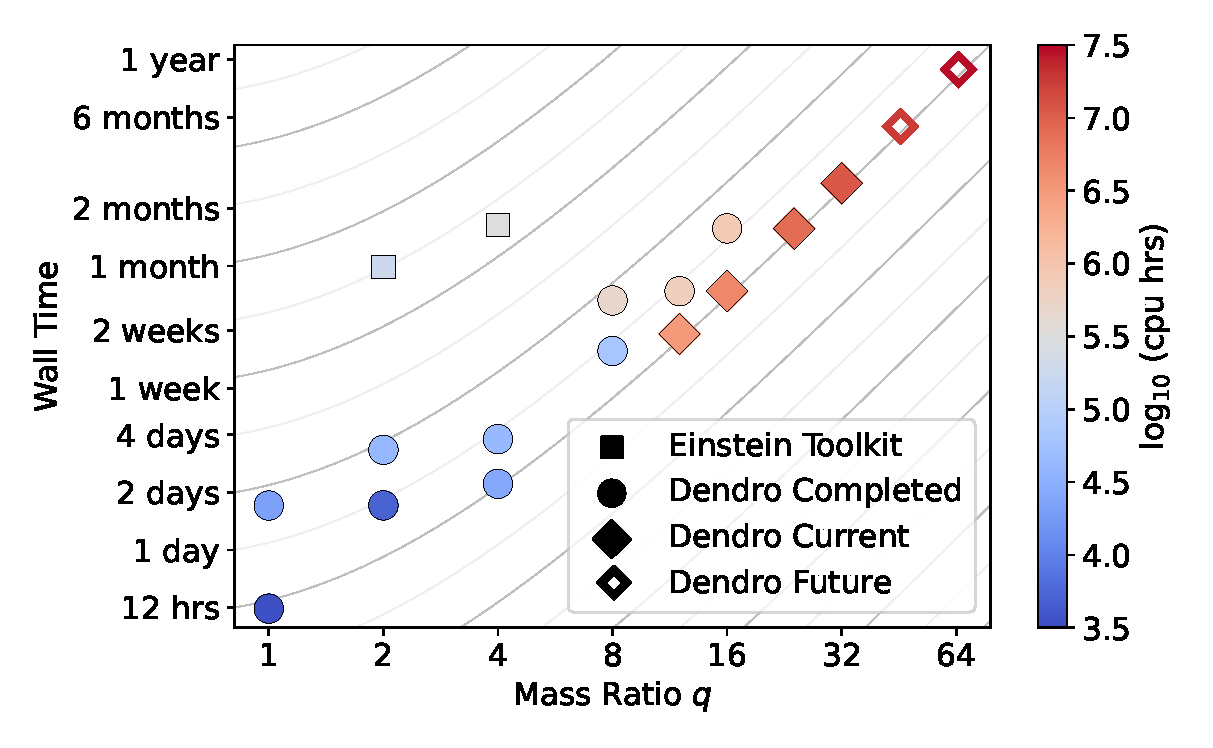
\includegraphics[width=0.8\textwidth]{Figures/walltime.pdf}
    \caption{Wall time of numerical relativity simulations as a function of mass ratio. As the mass ratio increases, the computational cost increases dramatically because the smaller black hole must be resolved with sufficient grid points. With current codes, performing a large number of high mass ratio simulations would therefore be prohibitively expensive.}
    \label{fig:walltime}
\end{figure}

To obtain more accurate waveforms, new techniques are needed: running existing codes at higher resolution will be insufficent. A drawback of the brute force approach simply increasing resolution is that the timesteps must also have a corresponding reduction. This, in turn, requires more timesteps, significantly increasing the total runtime and computational expense of the simulation.

One potential avenue for improving efficiency in numerical relativity codes lies in the computation of spatial derivatives. Most current implementations rely on explicit finite difference methods, while spectral methods although highly accurate are often difficult to implement. In this work, we explore compact finite difference (CFD) operators as an alternative. Compact schemes are implicit methods that can achieve higher spectral resolution than comparable explicit schemes \cite{Lele1992}. Across a variety of test problems, including the nonlinear sigma model, Maxwell's equations, and Einstein's equations, the compact finite difference schemes generally outperform the corresponding explicit methods.In some cases, the compact schemes achieve comparable accuracy to explicit schemes at approximately half the resolution. Despite their success in computational fluid dynamics and related fields, their use in numerical relativity remains limited \cite{Daszuta2023}.

In addition to the need for improved waveform modeling in GR, there is also a need for waveform models in alternative theories of gravity. Gravitational wave observations provide a powerful probe of gravity in the strongly nonlinear, dynamical regime, where deviations from general relativity (GR) may become apparent~\cite{Abbott2016,Abbott2025GWTC3GR,Yunes2025GWTests}. To search for such deviations, waveform templates from alternative theories of gravity are required~\cite{Yunes2009,Nair2019,Berti2015}. While studies have been carried out in theories such as Chern  Simons gravity~\cite{Alexander2009,Okounkova2019}, scalar  tensor theories~\cite{Barausse2013,Shibata2013,Berti2013,Palenzuela2014}, Einstein  Gauss  Bonnet gravity~\cite{Witek2019,Ripley2020b,East2021,Okounkova:2020rqw,Elley2022,Doneva2023sGB}, and Einstein  Maxwell  dilaton theory~\cite{Hirschmann2018,Julie2017}, waveform catalogs in these frameworks remain limited~\cite{Cardoso2012NRHEP,Corman2024NonlinearModificationsGR,Held2025}.


In this dissertation, we focus on Einstein  Maxwell  dilaton  axion (EMDA) theory. EMDA is of particular interest because it admits a well posed initial value formulation and arises as a low energy limit of string theory. In contrast to the no hair theorem in standard GR, which states that black holes can be completely defined by their mass spin and charge,  EMDA black holes possess additional degrees of freedom associated with the dilaton and axion fields.

We present a numerical relativity framework for simulating binary black hole mergers in EMDA theory. We analyze the resulting waveforms and investigate whether deviations from GR may be observable in gravitational wave signals.

\section{Background}
We focus on the study of black hole dynamics. As such, we begin with Einstein’s field equations:
\begin{equation}
    G_{ab} = 8 \pi T_{ab} + \Lambda g_{ab}.
\end{equation}
The left hand side describes the geometry of spacetime, while the right hand side encodes the matter and energy content.\cite{Wald1984,DInverno1992} We briefly examine each term in turn.

The tensor $G_{ab}$ is the Einstein tensor, which is constructed from quantities that encode the curvature of spacetime. The stress energy tensor $T_{ab}$ describes the distribution of matter and energy. The metric tensor $g_{ab}$ defines distances and the causal structure of spacetime. The constant $\Lambda$ is the cosmological constant, which is generally assumed to be very small. On the scales considered in this work, it is negligible, and we therefore set $\Lambda = 0$.

In standard general relativity simulations of binary black hole mergers, we consider vacuum spacetimes, for which
\begin{equation}
G_{ab} = 0.
\end{equation}
Although this equation appears innocuous, it represents a complex system of partial differential equations. In vacuum GR, these equations determine the spacetime geometry.

The Einstein tensor $G_{ab}$ is constructed from the Ricci tensor $R_{ab}$, the metric tensor $g_{ab}$, and the Ricci scalar $R$ according to
\begin{equation}
G_{ab} = R_{ab} - \frac{1}{2} g_{ab} R.
\end{equation}
The Ricci tensor and Ricci scalar are themselves contractions (contractions can be thought of as generalizations of dot products.) of the Riemann curvature tensor $R^{a}{} _{bcd}$. The Ricci tensor is obtained by contracting the first and third indices,
\begin{equation}
R _{ab} = R^{c}{} _{acb},
\end{equation}
and the Ricci scalar is obtained by a further contraction,
\begin{equation}
R = R ^{a}{}_{a}.
\end{equation}

The Riemann tensor is built from the Christoffel symbols and their derivatives. With our sign convention, it may be written as
\begin{equation}
R^{a}{}_{bcd}
=
\partial_c \Gamma^{a}{}_{bd}
- \partial_d \Gamma^{a}{}_{bc}
+ \Gamma^{a}{}_{ec}\Gamma^{e}{}_{bd}
- \Gamma^{a}{}_{ed}\Gamma^{e}{}_{bc},
\end{equation}
where $\Gamma^{a}{}_{bc}$ are the Christoffel symbols. These are determined by the metric and its first derivatives:
\begin{equation}
\Gamma^{a}{}_{bc}
=
\frac{1}{2} g^{ad}
\left(
\partial_b g_{dc}
+ \partial_c g_{bd}
- \partial_d g_{bc}
\right).
\end{equation}
Together, these relations show how the compact equation $G_{ab}=0$ encodes a system of nonlinear partial differential equations for the metric.

Although these geometric definitions expose the underlying structure of the Einstein equations, they still do not immediately resemble the second order system of partial differential equations used in numerical evolution. The equations can be reformulated into a strongly hyperbolic system suitable for time evolution, together with a set of equations that constrain the solution. We defer a complete discussion and expanation of how these evolution equations are formulated into a set of coupled partial differential equations to the Appendix~\ref{app:math_overview}. A key point though is that these constraint equations, such as the Hamiltonian and momentum constraints, must be satisfied by the initial data. In numerical simulations the constraints are not satisfied exactly because of finite resolution and truncation error. However, for a consistent numerical method, the constraint violations should decrease with increasing resolution and vanish in the continuum limit.

The preceding discussion is somewhat dense and we have skipped a few steps, so it is useful to consider a simpler example from Maxwell's equations. In vector notation, Maxwell's equations are
\begin{align}
\nabla \cdot \mathbf{E} &= 4\pi \rho, \\
\nabla \cdot \mathbf{B} &= 0, \\
\frac{\partial \mathbf{E}}{\partial t} &= \nabla \times \mathbf{B} - 4\pi \mathbf{J}, \\
\frac{\partial \mathbf{B}}{\partial t} &= - \nabla \times \mathbf{E}.
\end{align}

We present the full $3+1$ decomposition of Maxwell's equations in the Appendix~\ref{app:math_overview}. However, an important feature is already visible in this simpler form. There are eight scalar equations, but only six dynamical variables: $E_x$, $E_y$, $E_z$, $B_x$, $B_y$, and $B_z$. The remaining two equations constrain the allowed solutions.

Maxwell's equations can therefore be separated into evolution equations,
\begin{align}
\frac{\partial \mathbf{E}}{\partial t} &= \nabla \times \mathbf{B} - 4\pi \mathbf{J}, \\
\frac{\partial \mathbf{B}}{\partial t} &= -\nabla \times \mathbf{E},
\end{align}
and constraint equations,
\begin{align}
\nabla \cdot \mathbf{E} &= 4\pi \rho, \\
\nabla \cdot \mathbf{B} &= 0.
\end{align}

The constraint equations may also be written as
\begin{equation}
\mathcal{C}_E \equiv \nabla \cdot \mathbf{E} - 4\pi \rho = 0,
\end{equation}
\begin{equation}
\mathcal{C}_B \equiv \nabla \cdot \mathbf{B} = 0.
\end{equation}

These equations illustrate an important feature of many systems of partial differential equations. The electric and magnetic fields cannot be chosen arbitrarily. Instead, the initial data must satisfy the constraint equations before the evolution equations can be used to advance the solution in time. If the constraints are satisfied initially, they are preserved by the continuum evolution. In numerical simulations, finite resolution introduces small constraint violations, which should converge to zero as the resolution is increased.

General relativity has the same mathematical structure. Einstein's equations can be separated into evolution equations and constraint equations, and only initial data that satisfy the constraints represent physically valid solutions. Constructing such initial data is known as solving the Cauchy problem. More generally, the Cauchy problem is the initial value formulation of a system of partial differential equations, in which one specifies data on an initial spatial hypersurface that satisfy the constraint equations and then uses the evolution equations to determine the future development of the system.

Solving the Cauchy problem for Einstein's equations is nontrivial. In GR, the analogs of Gauss's law and the no monopole constraint are the Hamiltonian and momentum constraints. These constraints can be interpreted loosely as conditions related to energy and momentum conservation, and they must be satisfied by the initial data before the system can be evolved. Established techniques exist for constructing such data. In this work, we use the Bowen York equations to ensure that the initial data satisfy the momentum constraints. The Hamiltonian constraint then reduces to an elliptic equation that must be solved numerically. Further details on this procedure are given in the later chapters on initial data.

In EMDA theory, the Cauchy problem is further complicated by the presence of additional source terms. The stress energy tensor $T_{ab}$ encodes contributions from matter and nongravitational fields. In vacuum GR, this tensor vanishes, but in EMDA it includes contributions from the electromagnetic field, the dilaton, and the axion. Analytic single black hole solutions are known for special choices of the coupling parameters, such as $\alpha_0=\alpha_1=1$. However, numerical simulations allow us to vary these couplings and study how the resulting evolutions change. This dissertation addresses the challenges associated with constructing consistent initial data and evolving these systems numerically. For a more detailed discussion of the evolution equations and the mathematical machinery used to formulate them, see Appendix~\ref{app:math_overview}.

Once suitable initial data have been constructed and the system has been evolved, we extract the gravitational waveform. In this work, we compute the waveform using the Newman  Penrose formalism, in which outgoing gravitational radiation is represented by the Weyl scalar $\Psi_4$ \cite{Newman1962}. Details of how $\Psi_4$ is calculated are provided in Appendix~\ref{sec:appx:wave_extraction}.

The scalar $\Psi_4$ is related to the gravitational wave strain $h=h_+ i h_\times$ by
\begin{equation}
\Psi_4 = \frac{\partial^2 h}{\partial t^2},
\end{equation}
up to the sign conventions used for the null tetrad. From $\Psi_4$, we reconstruct the strain and compare simulated waveforms with one another and, in principle, with observed gravitational wave signals. To quantify the difference between two waveforms, we compute the mismatch:
we define the overlap and mismatch as:
\begin{equation}
    \mathcal{O}
    =
    \frac{
        \left|
        \langle h_1,h_2\rangle
        \right|
    }{
        \sqrt{
            \langle h_1,h_1\rangle
            \langle h_2,h_2\rangle
        }
    },
    \label{eq:app-waveex-time-overlap}
\end{equation}
The mismatch is then
\begin{equation}
    \mathcal{M}
    =
    1-\mathcal{O}.
    \label{eq:app-waveex-mismatch-basic}
\end{equation}
\begin{equation}
\mathrm{mismatch}(h_1,h_2) =    \max \mathcal{O}(h_1,h_2),
\end{equation}

where $\mathcal{O}$ is the normalized waveform overlap, and the maximum is taken over time shifts and polarization angles. The time shifts account for differences in the time of peak gravitational radiation, while the polarization angles account for rotations of the waveform polarization, equivalently phase rotations of the complex waveform.

The mismatch can be used to estimate the signal to noise ratio required to distinguish two waveforms. In the small mismatch limit, this distinguishability threshold is approximately
\begin{equation}
\rho \sim \frac{1}{\sqrt{2 \mathrm{mismatch}(h_1,h_2)}}.
\end{equation}
This estimate provides a useful way to interpret waveform differences, although it should not be regarded as an absolute detection criterion. In practice, interpreting differences between waveforms remains challenging because the parameter space is often degenerate. For example, it may not be immediately clear whether observed differences arise from spin, charge, or other physical effects.
Improving the accuracy of waveform comparisons requires improving the numerical simulations that produce the waveforms. We therefore also present our work incorporating compact finite difference operators into our numerical relativity code. To begin, we review the finite difference methods currently used in the code.

On a discrete grid, derivatives can be approximated using finite differences. For example, a second order accurate centered approximation to the first derivative is
\begin{equation}
\left.\frac{df}{dx}\right| _{i}
=
\frac{f _{i+1} - f_{i-1}}{2\Delta x}
+ \mathcal{O}(\Delta x^2).
\end{equation}

Higher order accurate formulas can be constructed by matching Taylor series expansions. For instance, a fourth order accurate centered stencil is
\begin{equation}
\left.\frac{df}{dx}\right| _{i}
=
\frac{-f _{i+2} + 8 f_{i+1} - 8 f_{i-1} + f_{i-2}}{12\Delta x}
+ \mathcal{O}(\Delta x^4).
\end{equation}
These finite difference approximations are standard tools for numerical solutions of partial differential equations \cite{BaumgarteShapiro2010}.

The above examples are explicit finite difference schemes, since the derivative at grid point $i$ is computed directly from nearby function values. Alternatively, one can approximate the first derivative using a compact, or implicit, finite difference scheme of the form
\begin{equation}
\beta f'_{i-2} + \alpha f'_{i-1} + f'_i
+ \alpha f'_{i+1} + \beta f'_{i+2}
=
c,\frac{f_{i+3} - f_{i-3}}{6\Delta x}
+ b,\frac{f_{i+2} - f_{i-2}}{4\Delta x}
+ a,\frac{f_{i+1} - f_{i-1}}{2\Delta x}.
\end{equation}
Here $f'_i$ denotes the numerical approximation to $df/dx$ at grid point $i$. Compact finite difference schemes of this type were developed to obtain higher spectral resolution than comparable explicit schemes \cite{Lele1992}.

The coefficients are determined by matching Taylor series expansions to the desired order of accuracy. For the above stencil, the consistency conditions include
\begin{align}
a + b + c &= 1 + 2\alpha + 2\beta,
&& \text{second order}, \\
a + 2^2 b + 3^2 c &= 2\frac{3!}{2!}\left(\alpha + 2^2\beta \right),
&& \text{fourth order}, \\
a + 2^4 b + 3^4 c &= 2\frac{5!}{4!}\left(\alpha + 2^4\beta \right),
&& \text{sixth order}.
\end{align}
This approach is more complex than an explicit finite difference stencil because the derivatives are obtained by solving an implicit system. The tradeoff is that compact schemes can provide improved accuracy and enhanced spectral resolution compared to explicit methods \cite{Lele1992}. This improvement in spectral resolution is illustrated in Fig.~\ref{fig:spectral_resolution}. There are many possible compact finite difference operators that can be constructed. In this work, we describe our methodology for identifying accurate and stable compact derivative operators and evaluate their performance relative to their explicit counterparts.

\begin{figure}[t]
\centering
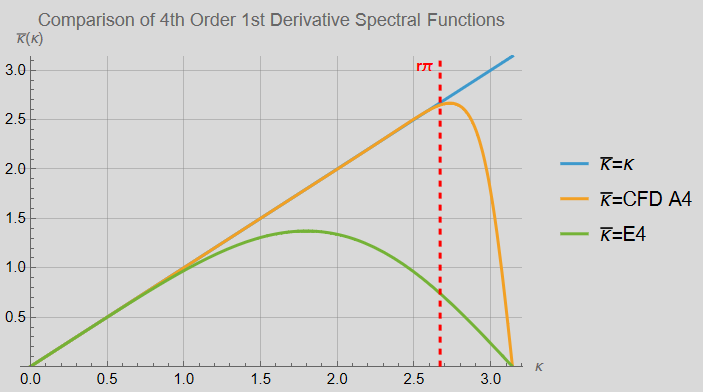
\includegraphics[width=0.8\textwidth]{Figures/1stDerivativeSpectralIntTest.png}
\caption{Spectral resolution of explicit and compact fourth order first derivative operators. The solid reference curve represents perfect resolution, and the dashed vertical line marks the cutoff frequency used in the optimization. The compact finite difference operator maintains better agreement with the ideal resolution curve over a wider range of wavenumbers.}
\label{fig:spectral_resolution}
\end{figure}

\section{Summary of Dissertation}

This dissertation primarily presents results from binary black hole simulations in Einstein  Maxwell  dilaton  axion (EMDA) theory, along with a study of compact finite difference methods for numerical relativity. The dissertation is organized as follows. Chapter~2 discusses the formulation of the initial data and presents results from head on collision simulations. Chapter~3 presents inspiral and merger results in EMDA theory. Chapter~4 explores interpolated EMDA models in which the coupling strengths are varied. Chapter~5 investigates the implementation of compact finite difference operators in numerical relativity codes.

Several of the results presented in this dissertation are currently in preparation for publication.

Each of these projects involved multiple collaborators. The EMDA work builds on earlier contributions by Hyun Lim at Los Alamos National Laboratory and was carried out collaboratively with Eric Hirschmann at Brigham Young University, David Van Komen at the University of Utah, Sebastian Vander Ploeg Fallon at Cornell University, and David Neilsen at Brigham Young University. The compact finite difference (CFD) project was conducted in collaboration with Eric Hirschmann, David Van Komen, David Neilsen, Nathaniel Garey, and Luke Papenfuss.

\section{Conventions}

In this work, we use geometrized units with $c=G=1$. Unless otherwise stated, lengths and masses are expressed in units of a characteristic mass scale $M$. In physical units, a length scale $d=M$ corresponds to $d=GM/c^2$, while a time scale $t=M$ corresponds to $t=GM/c^3$.

We use the metric signature $( ,+,+,+)$ and assume the Einstein summation convention unless otherwise stated. Spacetime indices $a,b,c,\ldots$ run over $0,1,2,3$, while spatial indices $i,j,k,\ldots$ run over $1,2,3$. The symmetric and antisymmetric parts of a tensor are defined as
\begin{equation}
T_{(ab)} \equiv \frac{1}{2}\left(T_{ab}+T_{ba}\right),
\qquad
T_{[ab]} \equiv \frac{1}{2}\left(T_{ab} T_{ba}\right).
\end{equation}

Partial derivatives are denoted by $\partial_i g$ or equivalently $g_{,i}$. Covariant derivatives are written as $\nabla_a f_b$ or equivalently $f_{b;a}$. The Lie derivative of a tensor $X^a$ along a vector field $\beta^a$ is denoted by $\mathcal{L}_{\beta}X^a$.

%In general, we use the following notation for geometric quantities. Objects associated with the spacetime manifold $\mathcal{M}$ are denoted by $g_{ab}$, ${}^{(4)}\Gamma^{a}{} _{bc}$, $\nabla_a$, ${}^{(4)}R _{ab}$, and related quantities. Objects associated with a spatial slice $\Sigma$ are denoted by $\gamma_{ij}$, $\Gamma^{i}{} _{jk}$, $D_i$, $R _{ij}$, and related quantities. Objects associated with a conformally related space are denoted by $\tilde{\gamma} _{ij}$, $\tilde{\Gamma}^{i}{} _{jk}$, $\tilde{D} _i$, $\tilde{R} _{ij}$, and related quantities.
